\documentclass[a4paper,11pt]{jsarticle}


% 数式
\usepackage{amsmath,amsfonts,amssymb}
\usepackage{bm}
% 画像
\usepackage[dvipdfmx]{graphicx}
\usepackage[dvipdfmx]{color}
\usepackage{siunitx}
\usepackage{wrapfig}
\usepackage{cases}
\usepackage{dcolumn}
\makeatletter
\newcommand{\figcaption}[1]{\def\@captype{figure}\caption{#1}}
\newcommand{\tblcaption}[1]{\def\@captype{table}\caption{#1}}
\makeatother

\usepackage{listings,jvlisting}
\lstset{
  basicstyle={\ttfamily},
  identifierstyle={\small},
  commentstyle={\smallitshape},
  keywordstyle={\small\bfseries},
  ndkeywordstyle={\small},
  stringstyle={\small\ttfamily},
  frame={tb},
  breaklines=true,
  columns=[l]{fullflexible},
  numbers=left,
  xrightmargin=0zw,
  xleftmargin=3zw,
  numberstyle={\scriptsize},
  stepnumber=1,
  numbersep=1zw,
  lineskip=-0.5ex
}


\begin{document}
\title{壁に立てかけた棒について}
\date{}
\maketitle

2021/5/26における自主ゼミにおいて、
ラグランジアンの説明を行った。
その際にラグランジアンにすでに作用点の情報が入っているとか議論になって結構面白かった。

\subsection{二重振り子の内力と外力}
実は二重振り子の天井の固定点にかかる力と振り子の間の力を同時に求めるときに、
\begin{lstlisting}
  Fx_in = -functionalDerivative(L, x2);
  Fy_in = -functionalDerivative(L, y2);
  
  Fx_out = -functionalDerivative(L, x1) + Fx_in;
  Fy_out = -functionalDerivative(L, y1) + Fy_in;
\end{lstlisting}
こんな風に計算したらうまくいったが、
これは
\begin{figure}[h]
  \centering
  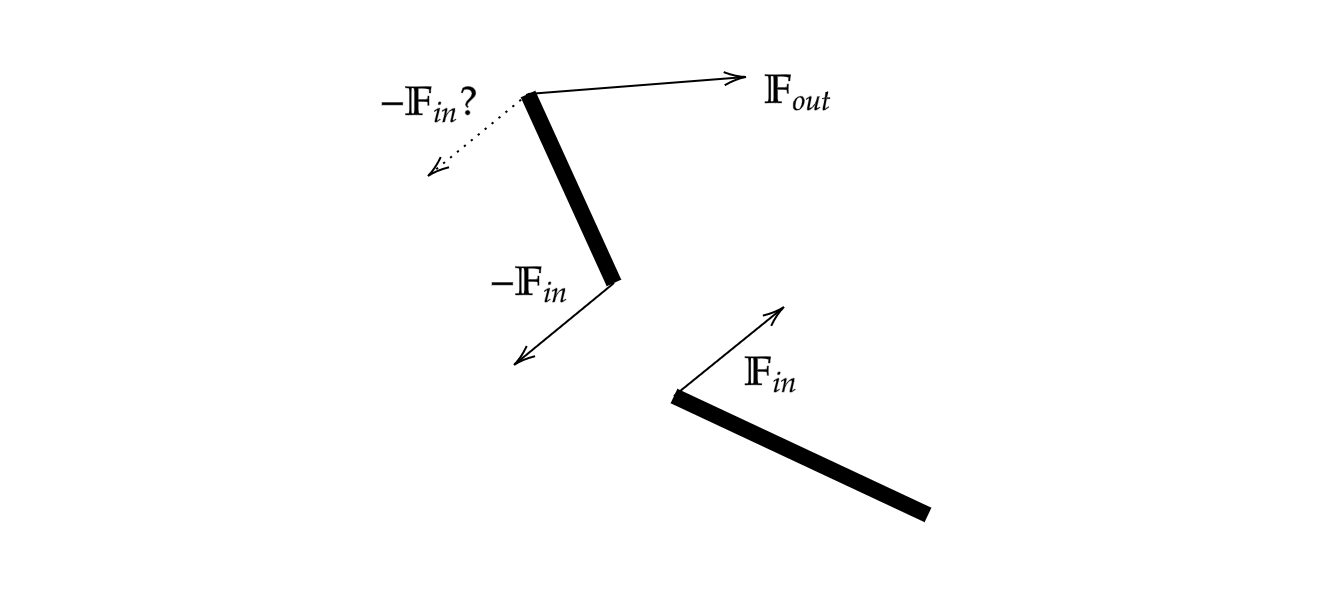
\includegraphics[width = 1\textwidth]{double_Stick.png}
  \caption{二重振り子と外力と内力}
  \label{fig:double_Stick}
\end{figure}
こんな感じで、
うまく求められている作用が分からない。
関節角度を絶対でとるか、相対でとるかの時にも他の間接トルクの作用とか考えた。
それに似てる。

図\ref{fig:double_Stick}みたいに、完全に分かれている状態を、
$x_{out}, x_{in}, L(x_{out},\dot{x}_{out},x_{in},\dot{x}_{in})$、
くっつけた状態を$x'_{out}, x'_{in}(x_{out})$とする。
くっつけてない状態において
\begin{align*}
  X_{out} &= \frac{d}{dt}\frac{\partial L}{\partial \dot{x}_{out}} - \frac{\partial L}{\partial x_{out}}
  \\ X_{in} &= \frac{d}{dt}\frac{\partial L}{\partial \dot{x}_{in}} - \frac{\partial L}{\partial x_{in}}
\end{align*}
と定義すると、これがちゃんと$\mathbb{F}_{out}, \mathbb{F}_{in}$の成分と一致する。
これをくっつけると、
\begin{align*}
  \frac{d}{dt}&\frac{\partial L(x_{out},\dot{x}_{out},x_{in},\dot{x}_{in})}{\partial \dot{x}'_{out}}
   - \frac{\partial L(x_{out},\dot{x}_{out},x_{in},\dot{x}_{in})}{\partial x'_{out}}
  \\ &= \frac{d}{dt}
  \left(\frac{\partial L}{\partial \dot{x}_{out}}\frac{\partial \dot{x}'_{out}}{\partial \dot{x}'_{out}}
   + \frac{\partial L}{\partial \dot{x}_{in}}\frac{\partial \dot{x}'_{in}}{\partial \dot{x}'_{out}}\right)
   - \left(\frac{\partial L}{\partial x_{out}}\frac{\partial x'_{out}}{\partial x'_{out}}
   + \frac{\partial L}{\partial x_{in}}\frac{\partial x'_{in}}{\partial x'_{out}}\right)
\end{align*}
てなる。これで$x'_{in} = x'_{out} + C$ということを考えれば、
\begin{align*}
  \frac{d}{dt}\frac{\partial L(x_{out},\dot{x}_{out},x_{in},\dot{x}_{in})}{\partial \dot{x}'_{out}}
   - \frac{\partial L(x_{out},\dot{x}_{out},x_{in},\dot{x}_{in})}{\partial x'_{out}}
   = X_{out} - X_{in}
\end{align*}
\begin{align*}
  \therefore X_{out} = \frac{d}{dt}\frac{\partial L}{\partial \dot{x}'_{out}}
  - \frac{\partial L}{\partial x'_{out}} + X_{in}
\end{align*}
となる。
だからちゃんとラグランジアンには作用点の情報が含まれている。
別々で計算して後で合わせるときはマジで気を付けないといけない。
下から順番に計算していくのが一番安全そうである。

\clearpage
\section{壁に立てかけた棒}
\begin{figure}[h]
  \centering
  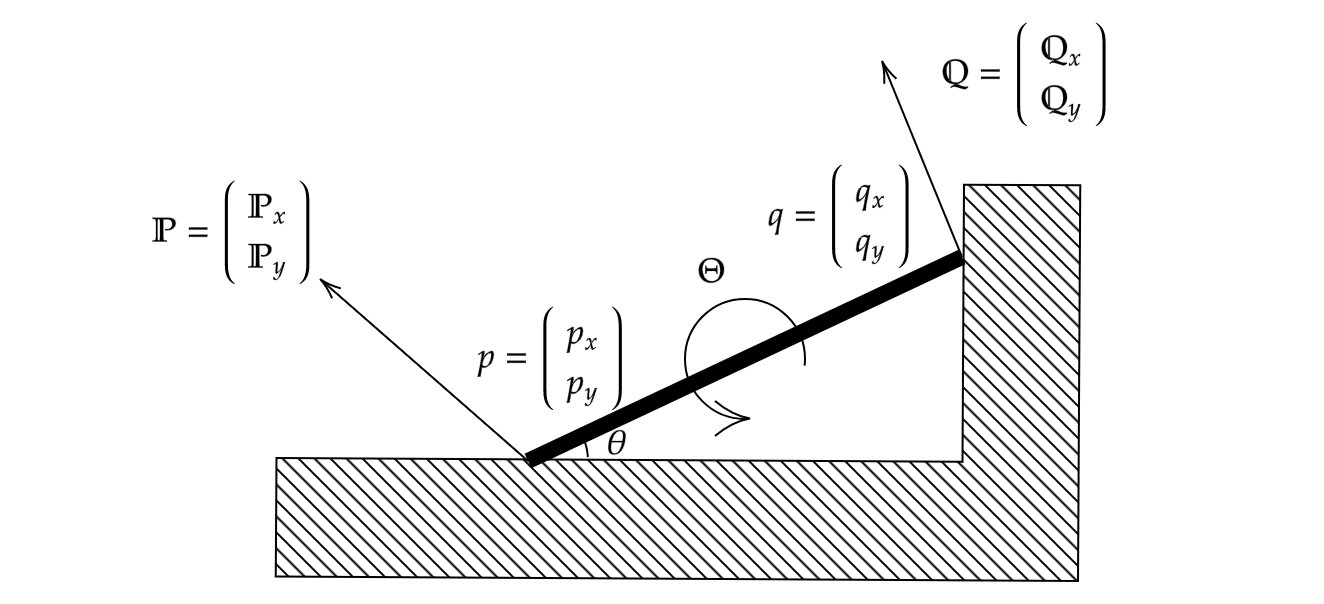
\includegraphics[width = 1\textwidth]{wall_And_Stick.png}
  \caption{壁に立てかけた棒}
  \label{fig:wall_And_Stick}
\end{figure}
今日の本題は、ラグランジアンによる運動方程式は変数の分しか存在しないことである。
図\ref{fig:wall_And_Stick}の状況において、
未知数になりうるものは$\ddot{p},\mathbb{P},\ddot{q},\mathbb{Q},\ddot{\theta},\Theta$の6つ。
でも今回は立てかけた棒なので、
$\ddot{p},\ddot{q},\ddot{\theta} = 0$
である。
つまり未知数は$\mathbb{P},\mathbb{Q},\Theta$である。
しかし、実際
\begin{align*}
  q = p + r\begin{pmatrix}
    \cos\theta \\
    \sin\theta
  \end{pmatrix}
\end{align*}
であるから、微分可能変数は$p,\theta$の2つである。
他のパターンとしては$(p,q), (q,\theta)$が存在する。
いずれにおいても微分可能変数は2つである。
つまり、
未知数$\mathbb{P},\mathbb{Q},\Theta$を求める式が足りない。

これが当たり前のことである、ということが本日の結論である。
この結論を説明する。

まず簡単な例でいえば、
立てかける棒にかかる力$\mathbb{P},\mathbb{Q}$を単純に求める際、
\begin{align*}
  0 &= \mathbb{P} + \mathbb{Q} \\
  0 &= (モーメントアーム)\times\mathbb{P}  + (モーメントアーム)\times\mathbb{Q}
\end{align*}
みたいに求める。
実はこれ、自然と$\Theta = 0$を前提としている。

また、実は$q$で微分できるんじゃないかとか考えるが、
\begin{align*}
  \frac{\partial L}{\partial q} = \frac{\partial L}{\partial r}\times \frac{\partial r}{\partial q}
   + \frac{\partial L}{\partial \theta}\times \frac{\partial \theta}{\partial q}
\end{align*}
のうちの$\displaystyle \frac{\partial \theta}{\partial q}$は計算できない。
なんか良く分かんない。

だから未知数$\mathbb{P},\mathbb{Q},\Theta$のうち、どれか1つを入力する必要がある。
実験的に言うと、入力がフォースプレートとなる。


\end{document}